\documentclass[12pt,a4paper]{article}
\usepackage[utf8]{inputenc}
\usepackage{amsmath}
\usepackage{amsfonts}
\usepackage{amssymb}
\usepackage{tikz-qtree}
\author{Yu-Ching Chen\\g3yuch\\999780651}
\title{CSC418\\A2}
\begin{document}
\maketitle
\section*{1}
${}$

a)

\begin{minipage}{0.3\textwidth}
$a = (2,3)$

$b = (1,2)$

$c = (3,-1)$
\end{minipage}
\begin{minipage}{0.3\textwidth}
$a' = (10,8)$

$b' = (8,-4)$

$c' = (2,0)$
\end{minipage}
\\

$A = \begin{bmatrix}
2 & 1 & 3\\
3 & 2 & -1\\ 
1&1&1\\
\end{bmatrix}
$

$A' = \begin{bmatrix}
10 & 8 & 2\\
8 & -4 & 0\\
1&1&1\\
\end{bmatrix}
$

$RA = A'$

$R = \begin{bmatrix}
a&b&c\\
d&e&f\\
g&h&i\\
\end{bmatrix}
$

$\begin{bmatrix}
a+3 b+c & a+2 b+c & 3 a-b+c\\
2 d+3 e+f & d+2 e+f & 3 d-e+f\\
2 g+3 h+i & g+2 h+i & 3 g-h+i
\end{bmatrix} = \begin{bmatrix}
10 & 8 & 2\\
8 & -4 & 0\\
1 & 1 & 1
\end{bmatrix}$

$a = 0,   b = 2,   c = 4,   d = 8,   e = 4,   f = -20,   g = 0,   h = 0,   i = 1$
	
$R = \begin{bmatrix}
0&2&4\\
8&4&-20\\
0&0&1\\
\end{bmatrix}
$
\\

b)
3 for 2D homography, 2 for rigid 2D transformation
\\

c)
If an acute triangle was sheared enough the centroid will be outside of the triangle where an acute's centroid would be inside therefore centroid is not preserved.

If an acute triangle was sheared to become an obtuse triangle the otho-center will not be preserved as the ortho-center will be outside the triangle.

\section*{2}
${}$

a) A camera lens is used to admit more light to the camera and concentrate to a smaller spot size. Focal Length is how much the image is magnified and aperture is how intense the light on the image.
\\

b)

Translation of (-2,-1,-3) to camera position
\\

Calculate Normal from point to camera and up vector to get x axis of camera.

$(-1,2,1) - (2,1,3) = (-3,1,-2)$


x = $\frac{(-3,1,2)}{\sqrt{3^2 + 1^2 + (-2)^2}}\times (0,1,0) = (- \sqrt{\frac{2}{7} }, 0, - \frac{3}{ \sqrt{14} })$

Rotate wold x axis to camera x axis, let Rx be the rotation needed

let $v_x = (1,0,0) \times (- \sqrt{\frac{2}{7} }, 0, - \frac{3}{ \sqrt{14} }) = (0,\frac{3}{\sqrt{14}},0)$

$Rx = \begin{bmatrix}
1&0&\frac{3}{\sqrt{14}}\\
0&1&0\\
-\frac{3}{\sqrt{14}}&0&1
\end{bmatrix} + \begin{bmatrix}
0	&0&\frac{3}{\sqrt{14}}\\
0&0&0\\
-\frac{3}{\sqrt{14}}&0&0
\end{bmatrix}^2 \frac{(1+\sqrt{\frac{2}{7}})}{\frac{9}{14}}$

$= \begin{bmatrix}
-\sqrt{\frac{2}{7}}&0&\frac{3}{\sqrt{14}}\\
0&1&0\\
-\frac{3}{\sqrt{14}}&0&-\sqrt{\frac{2}{7}}
\end{bmatrix}$
\\

Calculate normal from camera x axis and point to camera will give up y axis of camera.

$y = (- \sqrt{\frac{2}{7} }, 0, - \frac{3}{ \sqrt{14} }) \times \frac{(-3,1,2)}{\sqrt{3^2 + 1^2 + (-2)^2}} =  (\frac{3}{14}, \frac{13}{14},-\frac{1}{7})$

Rotate world y axis to camera y axis, Let Ry be the rotation needed

Let $v_y = (0,1,0) \times (\frac{3}{14}, \frac{13}{14},-\frac{1}{7}) = (-\frac{1}{7}, 0, -\frac{3}{14})$

$Ry = \begin{bmatrix}
1&\frac{3}{14}&0\\
-\frac{3}{14}&1&\frac{1}{7}\\
0&-\frac{1}{7}	&1
\end{bmatrix} +
\begin{bmatrix}
0&\frac{3}{14}&0\\
-\frac{3}{14}&0&\frac{1}{7}\\
0&-\frac{1}{7}	&0
\end{bmatrix}^2
\frac{(1-\frac{13}{14})}{\frac{13}{196}}$

$= \begin{bmatrix}
\frac{173}{182}& \frac{3}{14}& \frac{3}{91}\\
-\frac{3}{14}&\frac{13}{14}&\frac{1}{7}\\
\frac{3}{91}&-\frac{1}{7}& \frac{89}{91}
\end{bmatrix}$
\\

Aligning z axis is not needed as aligning x and y will ensure z is also aligned.

Therefore Given world space W, Transformation needed are:

RyRxTW =
$= \begin{bmatrix}
\frac{173}{182}& \frac{3}{14}& \frac{3}{91}\\
-\frac{3}{14}&\frac{13}{14}&\frac{1}{7}\\
\frac{3}{91}&-\frac{1}{7}& \frac{89}{91}
\end{bmatrix}$
$= \begin{bmatrix}
-\sqrt{\frac{2}{7}}&0&\frac{3}{\sqrt{14}}\\
0&1&0\\
-\frac{3}{\sqrt{14}}&0&-\sqrt{\frac{2}{7}}
\end{bmatrix}$
$\begin{bmatrix}
1&0&0&-2\\
0&1&0&-1\\
0&0&1&-3\\
0&0&0&1
\end{bmatrix}W
$



\section*{3}
${}$

$f(x,y,z) = (R- \sqrt{x^2 + y ^2})^2 + z^2 - r^2$

$ = R^2 -2R\sqrt{x^2 + y ^2} -r^2 + x^2 + y^2 + z^2$

Surface normal at point x y z by taking partial derivatives

$\frac{d}{dx} = x (2- \frac{2R}{\sqrt{x^2 + y^2}})$ 

$\frac{d}{dy} = y (2- \frac{2R}{\sqrt{x^2 + y^2}})$ 

$\frac{d}{dz} = 2z$

Then the normal at point x y z is $(x (2- \frac{2R}{\sqrt{x^2 + y^2}}), y (2- \frac{2R}{\sqrt{x^2 + y^2}}), 2z )$
\\

Then the explicit equation for the tangent plane at point $x_0, y_0, z_0$ is

$(x_0 (2- \frac{2R}{\sqrt{x_0^2 + y_0^2}})(x-x_0) + y_0 (2- \frac{2R}{\sqrt{x_0^2 + y_0^2}})(y-y_0)+ 2z_0(z-z_0) = 0$
\\

Let $x_1 = Rcos \lambda, y_1 = Rsin\lambda ,z_1  = r$ 

$f(x_1,y_1,z_1) = R^2 -2R\sqrt{(Rcos\lambda)^2 + (Rsin\lambda)^2} - r^2 + (Rcos\lambda)^2 + (Rsin\lambda)^2 + r^2 = 0$

Therefore parametric curve lies on surface.
\\

Tangent vector $q(\lambda) = (\frac{d}{d\lambda}R cos\lambda, \frac{d}{d\lambda}Rsin\lambda, \frac{d}{d\lambda}r) = (-Rsin\lambda, Rcos\lambda, r)$
\\

$(-Rsin\lambda (2- \frac{2R}{\sqrt{(-Rsin\lambda)^2 + (Rcos\lambda)^2}})(x-(-Rsin\lambda)) + Rcos\lambda (2- \frac{2R}{\sqrt{(-Rsin\lambda)^2 + (Rcos\lambda)^2}})(y-(Rcos\lambda))+ 2z_0(z-r) = 0$

Therefore the tangent vector lies on the tangent plane

\pagebreak

\section*{4}
${}$

a)
d does not need to be rendered as c will be rendered over it.
\\

b)

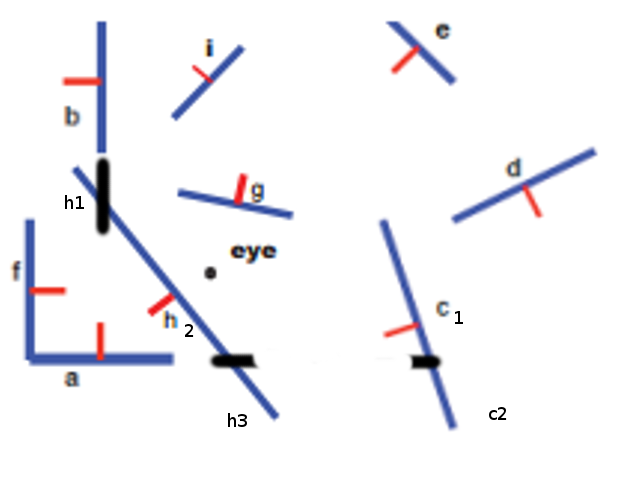
\includegraphics[scale=0.5]{question4}

\begin{tikzpicture}
\tikzset{n/.style={draw=none},
every tree node/.style={draw,circle, minimum size=2em},
    level distance=2cm,sibling distance=1cm}
\Tree
[.a 
	[.b
		[.f 
			[.$h_1$ ]
			\edge[n];[.\node[draw=none]{}; ]
		]
		[.$c_1$
			[.g
				[.i ]
				[.$h_2$ ]
			]
			[.d
				\edge[n];[.\node[draw=none]{}; ]
				[.e ]
			]
		]
	]
	[.$c_2$
		[.$h_3$
		]
		\edge[n];[.\node[draw=none]{}; ]
	]
]
\end{tikzpicture}

c)

($c_2, h_3$)a,(b,f,$h_1,c_1$,g,d,i,e,$h_2$)

$c_2,h_3$,a,(b,f,$h_1,c_1$,g,d,i,e,$h_2$)

$c_2,h_3$,a,(f,$h_1$),b,($c_1$,g,d,i,e,$h_2$)

$c_2,h_3$,a,f,$h_1$,b,($c_1$,g,d,i,e,$h_2$)

$c_2,h_3$,a,f,$h_1$,b,(d,e),$c_1$,(g,i,$h_2$)

$c_2,h_3$,a,f,$h_1$,b,d,e,$c_1$,(g,i,$h_2$)

$c_2,h_3$,a,f,$h_1$,b,d,e,$c_1$,i,g,$h_2$

\end{document}